Let us now continue our discussion of path integral quantization. Heuristically, we'll \begin{verbatim}import\end{verbatim} the details of path integral quantization and see what works out. We want to understand how to make sense of expressions like
\begin{equation}
    \int \cD h \cD X \,e^{iS[h,X]}
\end{equation}
where we are integrating over the space of metrics $h_{ab}$ and embedding fields $X^\mu$s. When we do this calculation, we have to be careful not to overcount-- there is a huge diffeomorphism symmetry and a Weyl symmetry in our theory relating physically equivalent states. If this path integral is to give us anything physically meaningful, we need to ``quotient out'' by the space of diffeomorphisms and Weyl transformations.

We would like to split the integral over all $h_{ab}$ into integrals over physically inequivalent $h_{ab}$ and those related by gauge transformations. Schematically,
\begin{equation}
    \cD h = \cD h_{\text{phys}}\times \mathcal{J}\cD h_{\text{Diff}\times \text{Weyl}},
\end{equation}
where $\mathcal{J}$ is a Jacobian factor whose importance we'll see in the following example.

\begin{exm}
    As a toy example, consider the following integral:
    \begin{equation*}
        \int dxdy\, e^{-(x^2 +y^2)}.
    \end{equation*}
    But notice that $x^2+y^2$ is invariant under rotations about the origin. When we pass to polar coordinates, the $\theta$ angular integral becomes totally trivial, so we might really be interested in this integral modulo rotations. Thus our integral can be rewritten
    \begin{equation*}
        \int d\theta \int dr \, re^{-r^2}.
    \end{equation*}
    This $\int d\theta$ will always give us a factor of $2\pi$ (the  ``volume'' of an orbit of the rotation group)-- the real interest is in the $dr$ integral.
\end{exm}

In this example, we needed the Jacobian of the coordinate transformation: $dxdy=rdr d\theta$. The same is true of our path integral. Formally, we will take
\begin{equation}
    \frac{1}{|\text{Diff}|\times |\text{Weyl}|}\int \cD h \cD X = \int \cD h_{\text{phys}}\cD S_{\text{phys}} \,\mathcal{J},
\end{equation}
where $\mathcal{J}$ is now a functional determinant and $|\text{Diff}|, |\text{Weyl}|$ represents the orbits of diffeomorphisms and Weyl transformations.
%
In the same way we could write
\begin{equation}
    \sqrt{\frac{\pi}{\det M}}=\int_V dx \,e^{-(x,Mx)},
\end{equation}
we will write $\mathcal{J}$ as a functional integral,
\begin{equation}
    \cJ =\int \cD b \cD c\, e^{-S[b,c]}.
\end{equation}

\subsection*{Global properties of the worldsheet} We need to know more about what type of worldsheets appear in the path integral. This will take us on a crash course through Riemann surfaces.

We have looked at 2-dimensional Riemannian manifolds $(\Sigma,h)$ modulo Weyl transformations. The set of Riemannian manifolds modulo Weyl transformations is known as \term{Riemann surfaces}. Quotienting out by diffeomorphisms is assumed. Note that worldsheets are Riemann surfaces.

We'll state a number of results without proof, though some of them are not too hard to prove-- for more detail, see Farkas and Kra, and also Donaldson.

The first idea we'll consider is the \term{worldsheet genus}. For Riemann surfaces without boundary (i.e. a closed string, neglecting the initial and final string states), the relevant topological data is encoded in the \term{Euler characteristic},
\begin{equation}
    \chi = \frac{1}{4\pi} \int_\Sigma d^2 \sigma \,\sqrt{h} R(h).
\end{equation}
Here, $R(h)$ is the Ricci scalar with respect to the worldsheet metric $h$. The Euler characteristic captures the idea that while we can locally make the metric look however we want, in general there will be obstructions to globally bringing the metric to a required form. The \term{genus} $g$ is given by
\begin{equation}
    \chi = 2-2g,
\end{equation}
and informally counts the ``number of holes in $\Sigma$,'' as shown in Fig. \ref{fig:riemanngenus}. Why we care is because the genus is a topological invariant-- we can't change the number of holes in a Riemann surface under smooth maps.

\begin{figure}
    \centering
    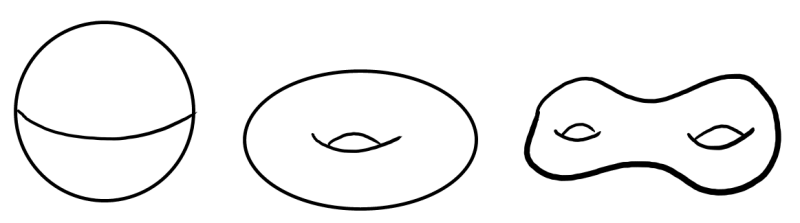
\includegraphics[width=0.75\textwidth]{2019/02/20190201_genus.png}
    \caption{Three surfaces of genus $0,1,$ and $2$, respectively. The first is the sphere $S^2$, the second is the torus $T^2$, and the final is a ``handlebody'' of genus two.}
    \label{fig:riemanngenus}
\end{figure}

\subsection*{Moduli space of Riemann surfaces} For a given genus $g$, the space of metrics on $\Sigma_g$ modulo Weyl and diffeomorphisms is a finite-dimensional space called the \term{moduli space}. Schematically,
\begin{equation*}
    \cM_g = \frac{\set{\text{metrics }h_{ab}}}{\set{\text{Diff}}\times \set{\text{Weyl}}}.
\end{equation*}
Both the numerator and denominator here are infinite dimensional, but our saving grace will be the following fact-- the integral itself is finite-dimensional.

A useful result is the following: let $s$ be the real dimension of the moduli space $\cM_g$. Then
\begin{equation}
    s=\dim \cM_g =\begin{cases}
    0, & g=0\\
    2, & g=1\\
    6g-6, & g\geq 2.
    \end{cases}
\end{equation}

\begin{exm}
    Given a metric $\hat h_{ab}$ on a $g=0$ surface, we can bring any metric to the form $e^{2w}\hat h_{ab}$. This is not the case for a torus ($g=1$). We can build a torus by imposing identifications on $\CC,$ i.e. under the equivalence relation
    \begin{equation}
        z\sim z + n \lambda_1 + m\lambda_2,
    \end{equation}
    where $n,m\in \ZZ$ and $\lambda_1,\lambda_2$ specify the ``dimensions'' of the torus.
    
    One can show that the ratio $\tau\equiv \lambda_1/\lambda_2$ is Diff and Weyl invariant. However, we can always choose $\lambda_1,\lambda_2$ such that $\Im (\tau)\geq 0$. We also get a metric
    \begin{equation}
        ds^2=\abs{dz+\tau d\bar z}^2.
    \end{equation}
    If we transform $\begin{pmatrix}\lambda_1 \\ \lambda_2\end{pmatrix}\to U\begin{pmatrix}\lambda_1 \\ \lambda_2\end{pmatrix}$ for some matrix $U$, then we can undo that change by also changing the equivalence relation numbers $(n,m)\to (n,m)U^{-1}$. For $n,m$ to be integers under any such transformation, we require the entries of $U$ to all be integers, i.e. $U\in SL(2,\ZZ)$.
    
    Our moduli space is
    \begin{equation}
        \cM_1 = \frac{UHP}{SL(2,\ZZ)},
    \end{equation}
    with $UHP$ the upper half-plane, $\tau,\Im \tau \geq 0$.
\end{exm}